\documentclass[UTF8,a4paper]{ctexart}
\usepackage[utf8]{inputenc}
\usepackage{amsmath}
\usepackage{pdfpages}
\usepackage{graphicx}
\usepackage{wrapfig}
\usepackage{listings}
\usepackage{multicol}
\newcommand{\tabincell}[2]{\begin{tabular}{@{}#1@{}}#2\end{tabular}}
\title{实验三\ \ 负反馈电路仿真及实验}
\author{张蔚桐\ 2015011493\ 自55}
\begin {document}
\maketitle
\section{预习任务}
\subsection{两级放大电路的恢复性调试}
这里我们回顾一下两级放大电路在仿真和实验中的性能指标

\begin{table}
\centering
\caption{两级放大电路在仿真和实验中的性能指标}
\begin{tabular}{|c|c|c|c|}
\hline 
测试情况 & 放大倍数$A_u$ & 输入电阻$R_i$ & 输出电阻$R_o$\\
\hline 
仿真 & -168 & $91\mathrm{k}\Omega$ & $3.08\mathrm{k}\Omega$ \\
\hline 
实际电路 & -155 & $91.6\mathrm{k}\Omega$ & $3.08\mathrm{k}\Omega$ \\
\hline 
\end{tabular}
\end{table}
\subsection{两级放大电路电压并联负反馈电路的设计}
\begin {wrapfigure}{r}{0pt}
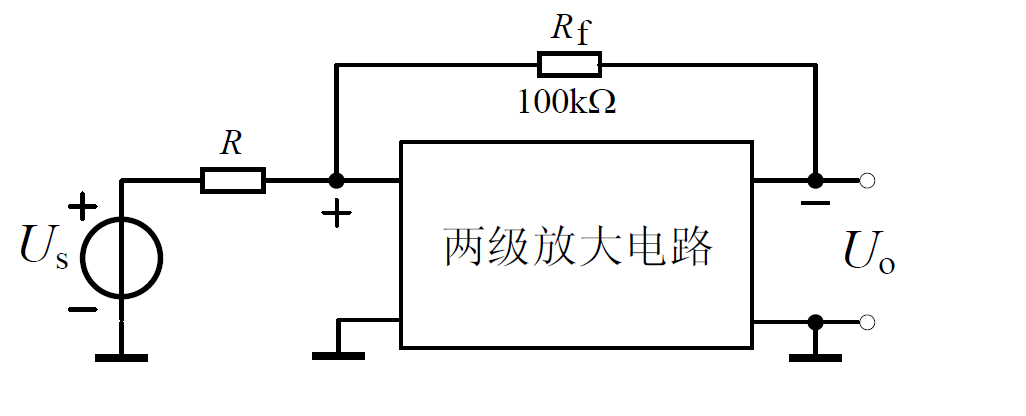
\includegraphics [width=60mm]{circuit.png}
\caption{实验用电路图}
\label{Circ}
\end {wrapfigure}
如图\ref{Circ}所示是实验用电路图,首先进行理论计算

若电路引入深度负反馈,则有
$$ A_{usf}\approx \frac{1}{FR}=-\frac{R_f}{R}=-10$$
可以立即解得$R=-\frac{R_f}{A_{usf}}=10\mathrm{k}\Omega$

同时计算深度负反馈条件得到
$$1+A_uF=1+A_u\frac{R_i}{R_f}\approx154 >>1$$

满足负反馈条件

同时进一步有,因为引入电压并联负反馈,输入电阻减小为
$$R_{if}=\frac{R_i}{1+AF}=591\Omega$$
输出电阻减小为
$$R_{of}=\frac{R_o}{1+AF}=20\Omega$$
\subsection{仿真测试}
仿真按照设计的要求完成电路的设计,得到的电路如图\ref{ACT}所示,相关的静态工作点已经标注在图中,我们得到$I_{CQ}=I_{DQ}=2\mathrm{mA}$,同时得到

\begin{figure}
\centering
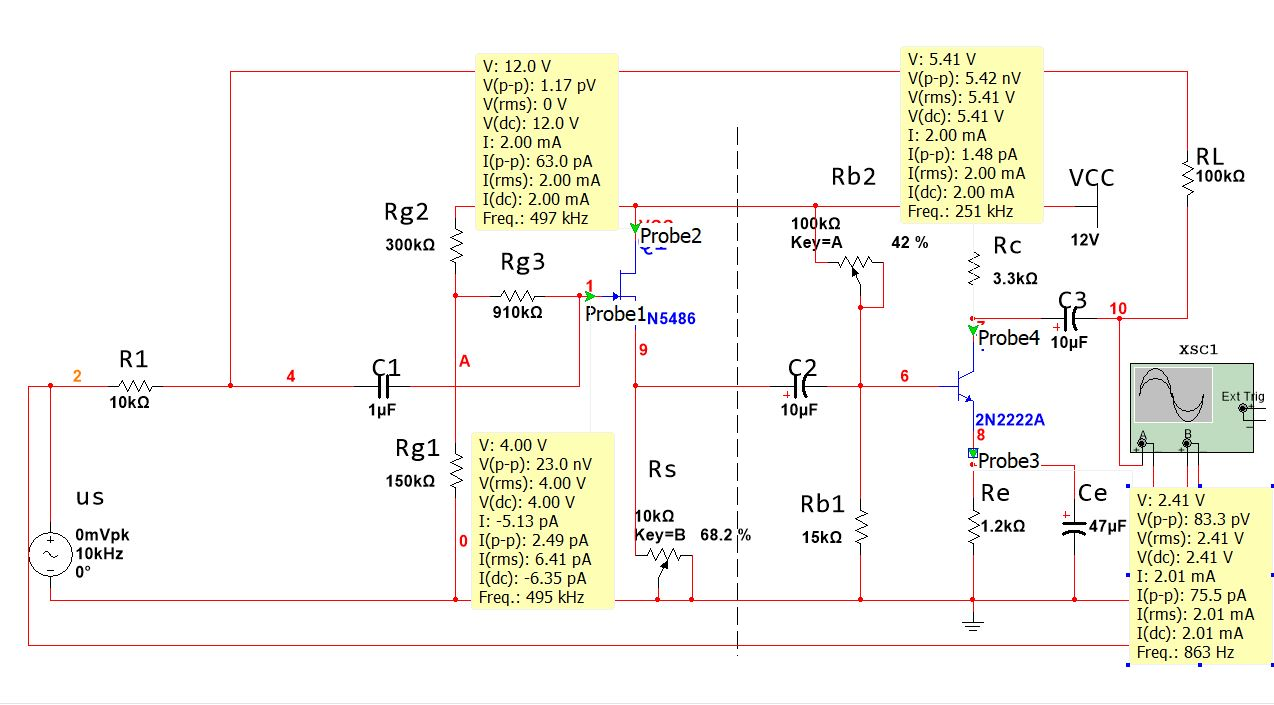
\includegraphics[width=\textwidth]{cir.jpg}
\caption{实验电路}
\label{ACT}
\end{figure}
\begin{figure}
\centering
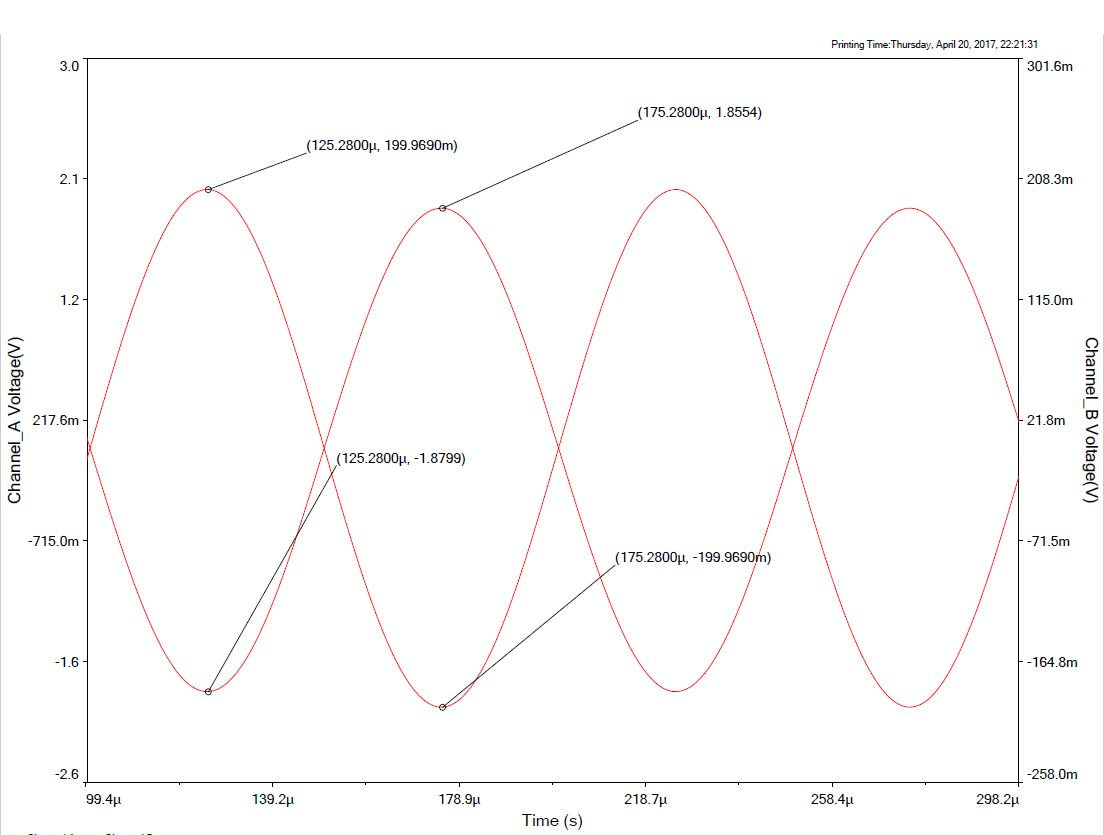
\includegraphics[width=\textwidth]{A.jpg}
\caption{负载开路放大倍数测试}
\label{A}
\end{figure}
所示,相关的静态工作点已经标注在图中,我们得到$I_{CQ}=I_{DQ}=2\mathrm{mA},U_{GDQ}=-8\mathrm{V},U_{CEQ}=3\mathrm{V}$满足题目中给定的要求

进一步按照题目中设置信号源幅度为200mV,频率为10kHz,得到电压放大倍数为如图\ref{A}所示,并且得到
$$A_{usf}=-\frac{1878.9+1855.4}{199.97+199.96}=-9.34\approx -10$$
和题目要求相近,同时测得负载开路输出电压峰峰值为$U_{o0}\approx1866\mathrm{mV}$

同时采用串联电阻法测量输入电阻,如图\ref{R}所示,可以计算得到输入电阻为
$$R_i\frac{28.5\mathrm{mV}}{37.1\mu\mathrm{A}}=768\Omega$$
输出电阻为$$R_o=\frac{1878.9+1855.4-3680\mathrm{mV}}{368\mu\mathrm{A}}=147\Omega$$
同时,在$10\mathrm{k}\Omega$负载电阻下$A_{usf}=-9.2$基本的变化趋势和理论估算的是一致的。

同时可以得到辐频特性曲线如图\ref{F}所示。可以看出低频截止频率约为17Hz,高频截止频率约为9.6MHz,但是在4MHz以上已经不稳定。

\begin{figure}
\centering
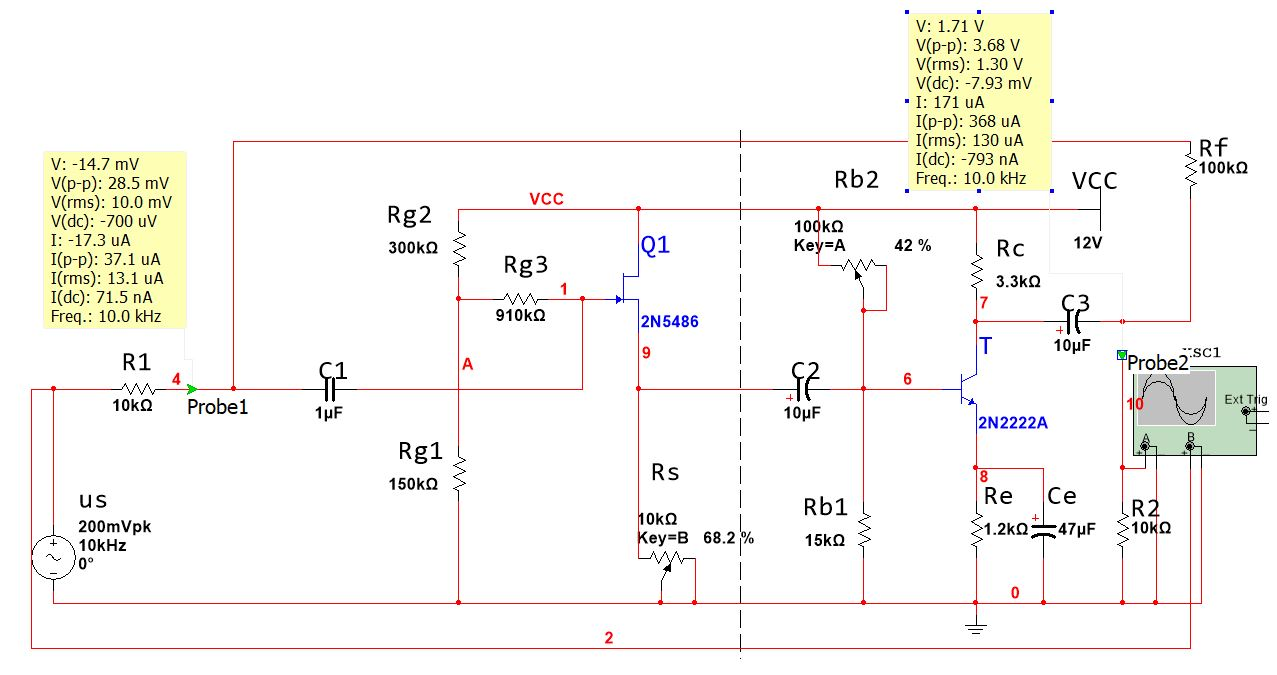
\includegraphics[width=\textwidth]{R.jpg}
\caption{输入输出电阻测试图}
\label{R}
\end{figure}

\begin{figure}
\centering
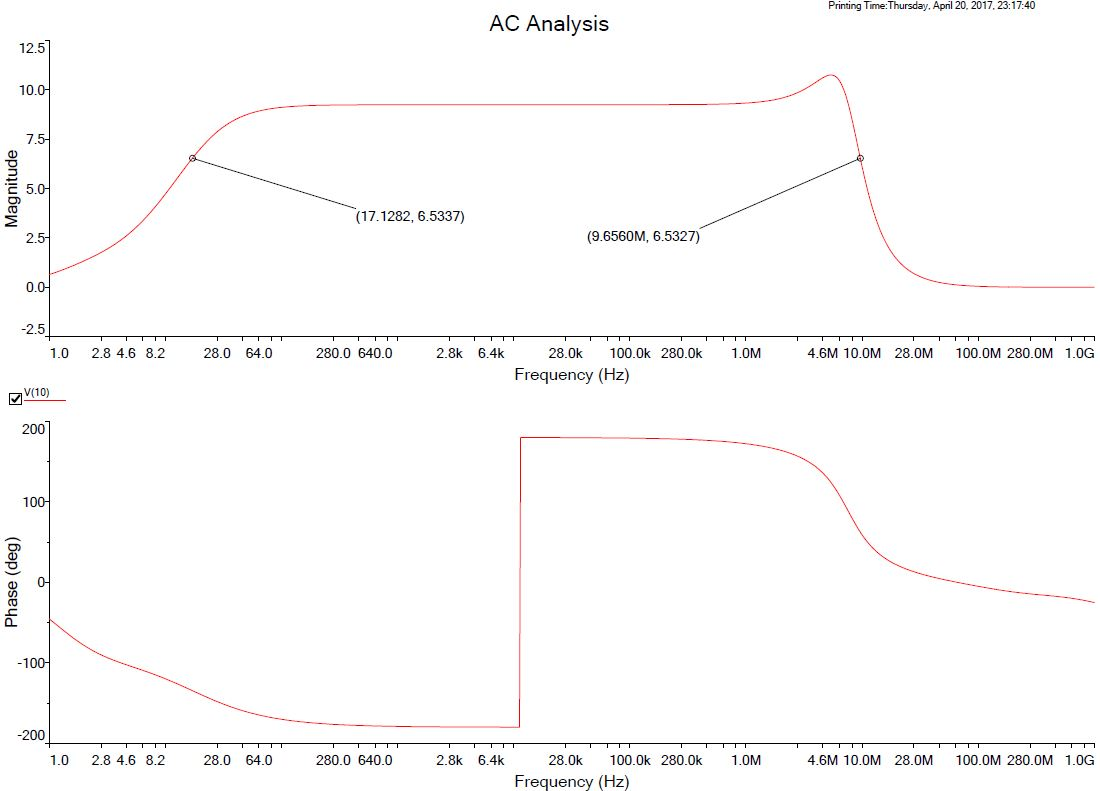
\includegraphics[width=\textwidth]{F.jpg}
\caption{辐频响应特性图}
\label{F}
\end{figure}
\section{电流并联负反馈的电路理论估计}

\begin{figure}
\centering
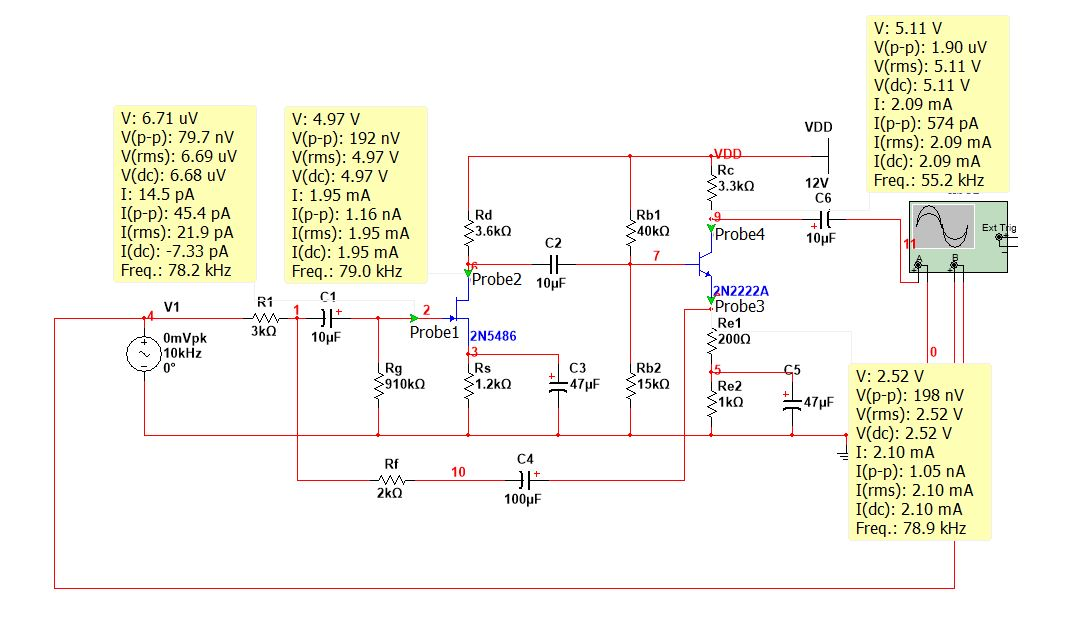
\includegraphics[width=\textwidth]{Q2.jpg}
\caption{电路图和静态工作点的测量}
\label{Q2}
\end{figure}
\begin{figure}
\centering
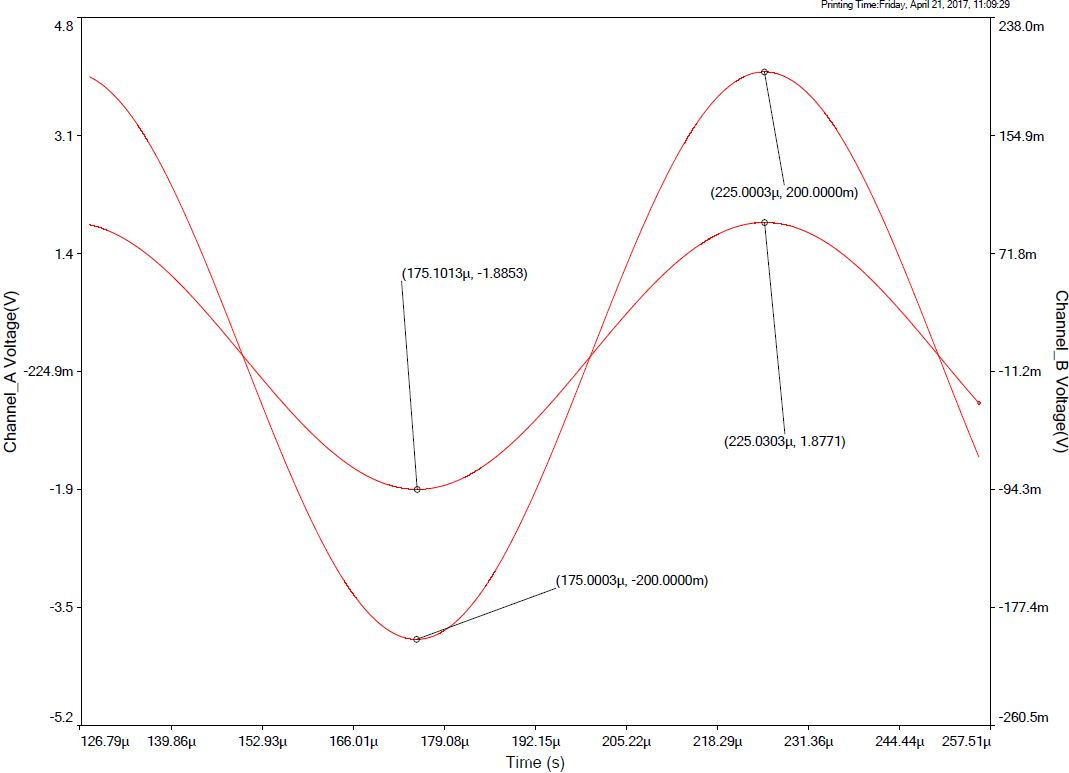
\includegraphics[width=\textwidth]{A2.jpg}
\caption{负载开路时输出电压放大倍数的测试}
\label{A2}
\end{figure}
\begin{figure}
\centering
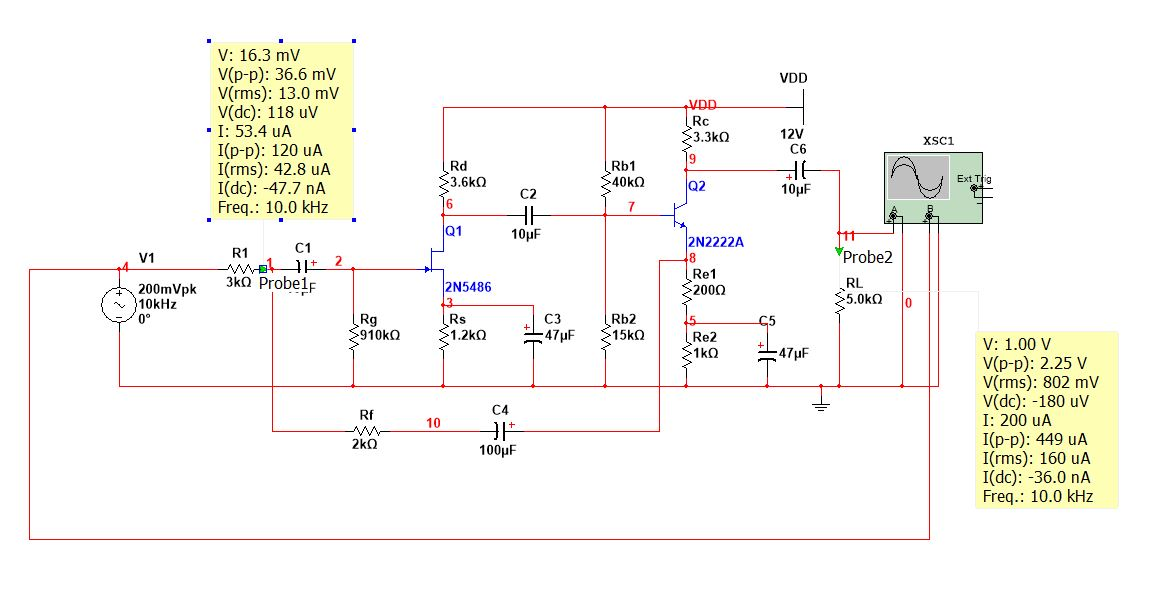
\includegraphics[width=\textwidth]{R2.jpg}
\caption{输入输出电阻的测量}
\label{R2}
\end{figure}
\end{document}
